\documentclass{article}

\usepackage{lipsum}
\usepackage[margin=2cm, left=2cm, includefoot]{geometry}
\usepackage{graphicx}
\usepackage{float}
\usepackage{hyperref}

% Header and footer
\usepackage{fancyhdr}
\pagestyle{fancy}

\rhead{}
\lhead{}
\fancyfoot{}
\fancyfoot[R]{\thepage}
\renewcommand{\headrulewidth}{0pt}
\renewcommand{\footrulewidth}{0pt}
%

\begin{document}

\begin{titlepage}
	\begin{center}
		\line(1,0){400}\\
		[6mm]
		\huge{\bfseries PROJECT TENDER}\\
		[2mm]
		\line(1,0){400}\\
		[5mm]
		\large\textbf{PROJECT:}\\\textsc{Drone Mission Control - Agile}\\
		[3mm]
		\large\textbf{CLIENT:}\\\textsc{Retro Rabbit}\\
		[3mm]
		\large \textbf{TEAM:}\\\textsc{Funge}\\
		\line(1,0){400}\\
		[5mm]
		\large \textbf{Team Members:}\\
		[3mm]
		\large Matthew Botha\\
		\large Gian Paolo Buffo\\
		\large Matthias Harvey\\
        \large Dillon Heins\\[3mm]
		\begin{figure}[H]
			\centering
			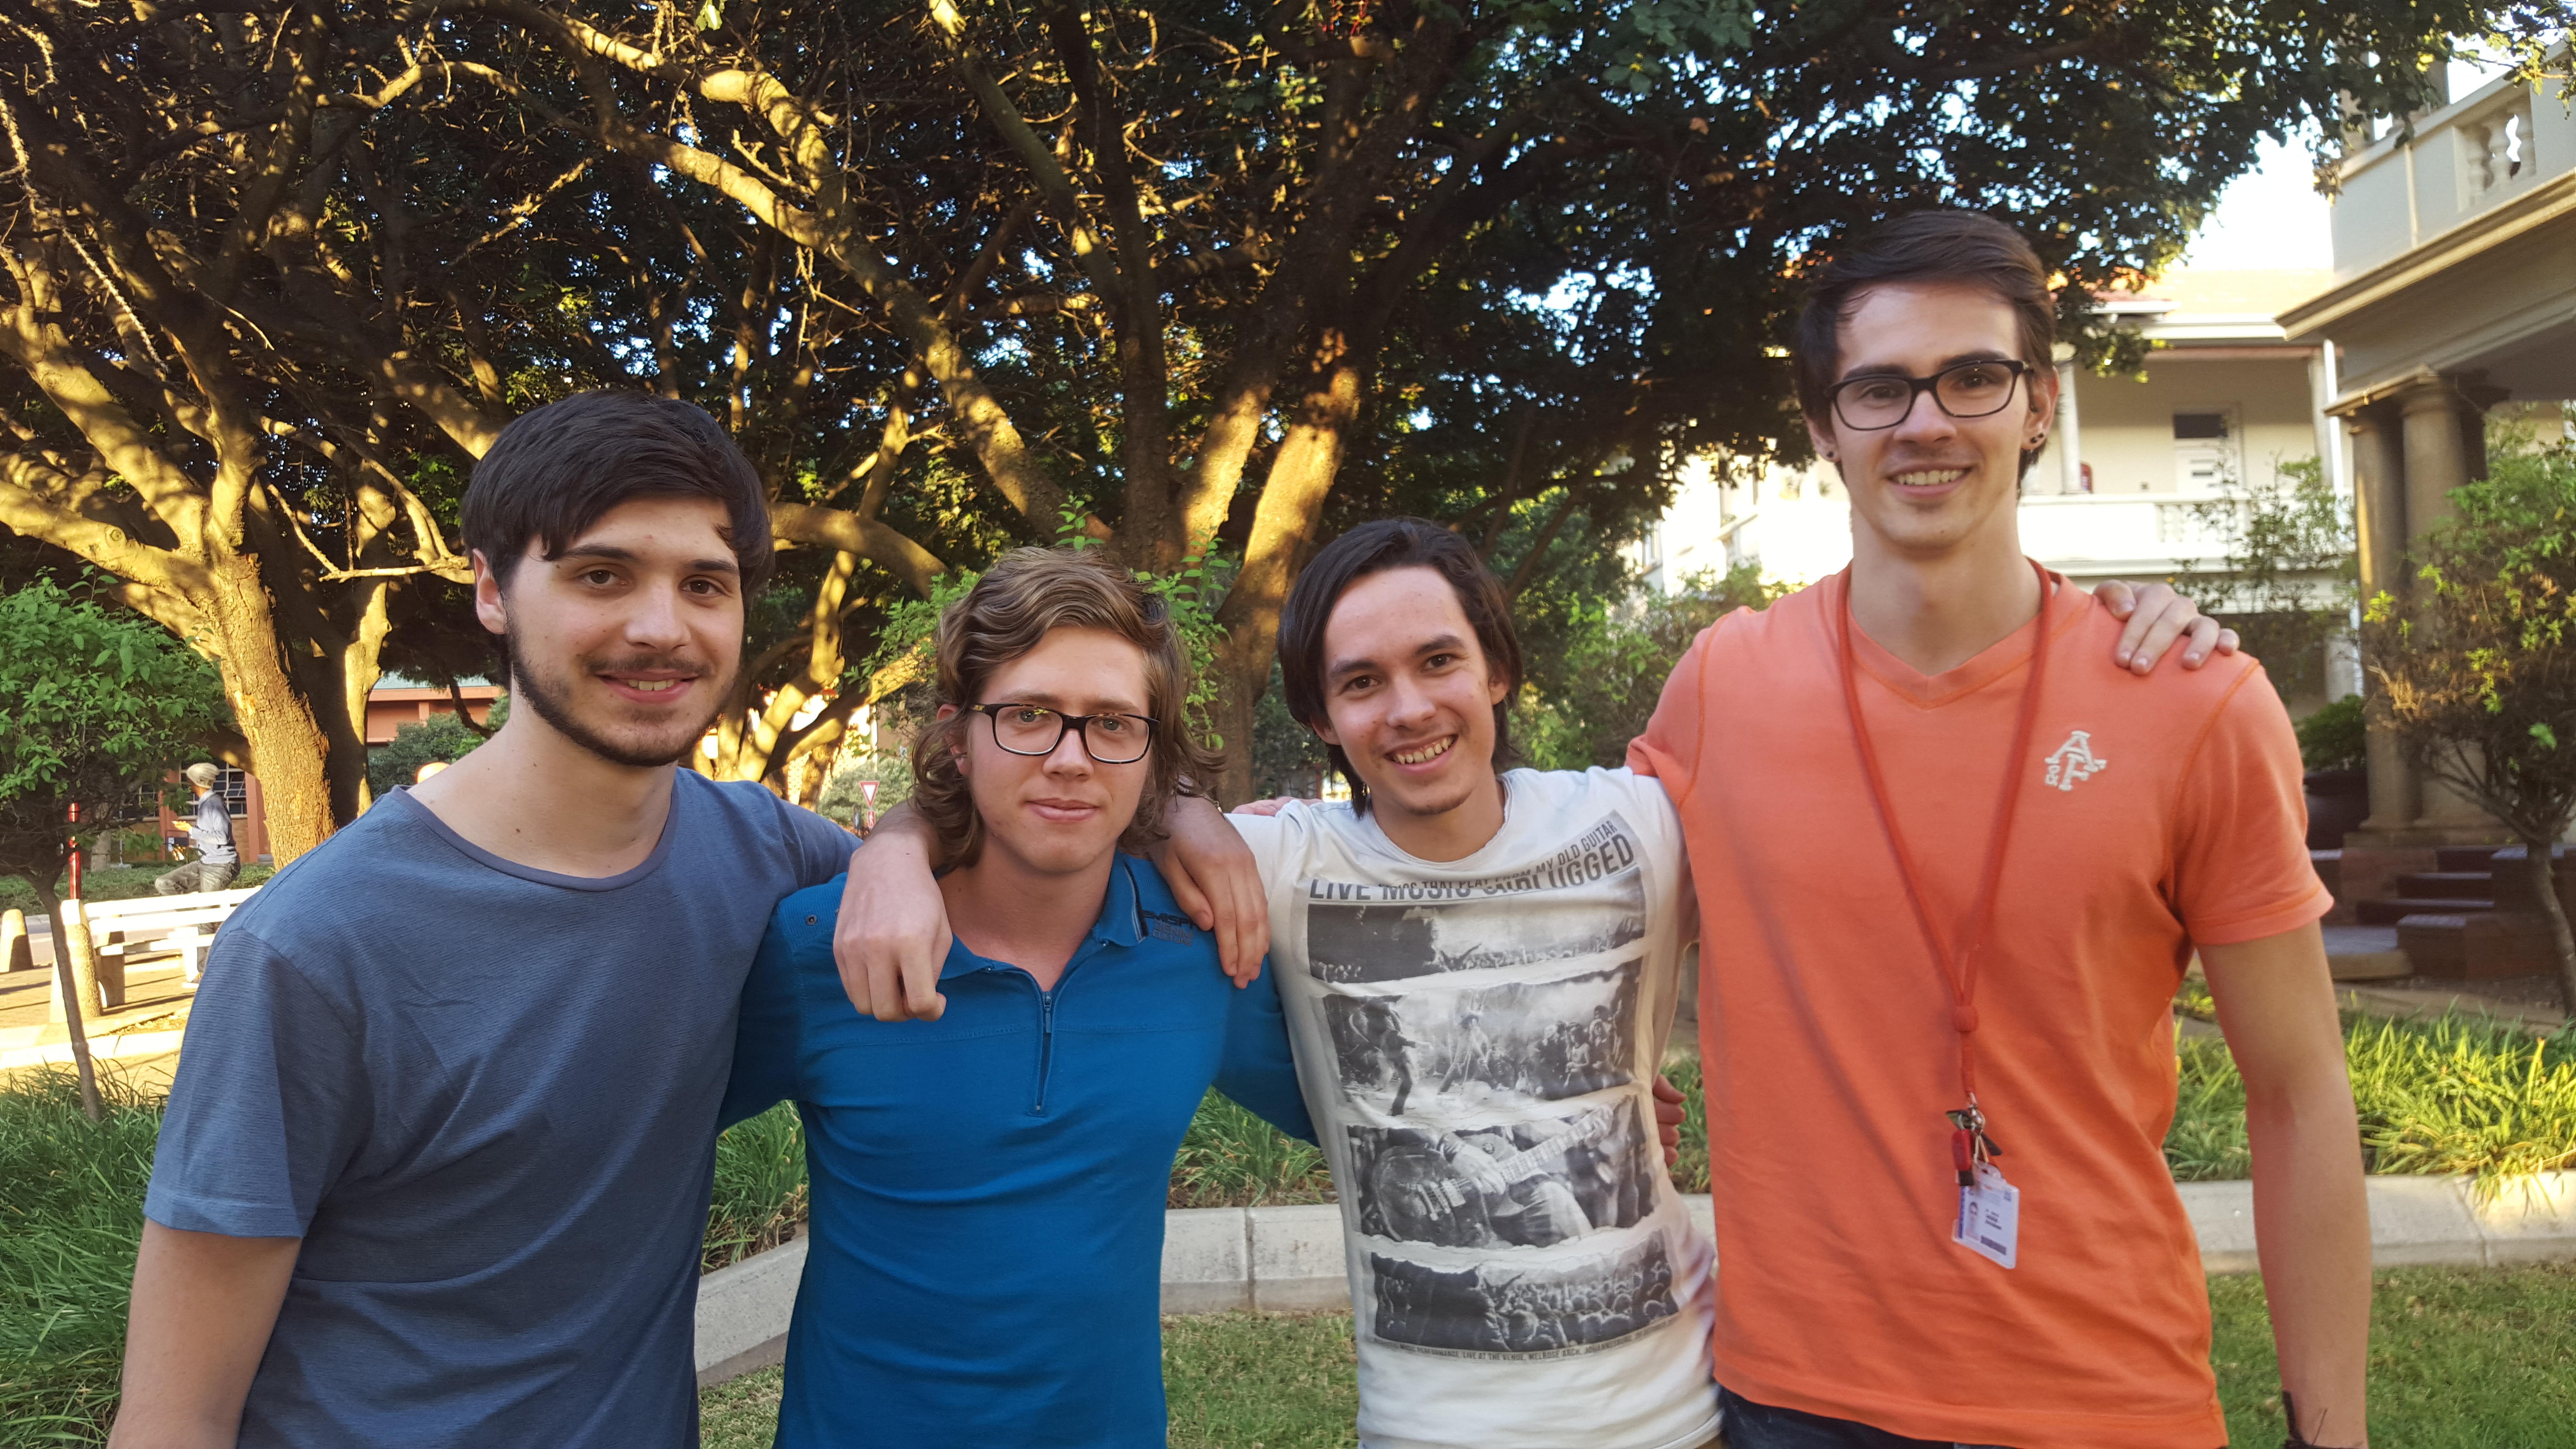
\includegraphics[width=0.8\textwidth]{../teamPhoto.jpg}
			\caption{Matthew Botha, Matthias Harvey, Gian Paolo Buffo, Dillon Heins}
		\end{figure}
    \end{center}

	\vspace{7mm}

    \begin{flushright}
        \textsc{\large Department of Computer Science\\
        University of Pretoria\\
        01 May 2016\\}
    \end{flushright}
\end{titlepage}

\section{The Team}
\subsection{Matthew Botha}
\textbf{Profile:}\\
I am fascinated by all things technological and love tinkering with new gadgets and technology. I am interested in artificial intelligence, especially in computer security systems, as well as computer networks and the Internet of Things. I am an avid reader and enjoy cooking and playing guitar.
\subsubsection{Contact}
\begin{itemize}
	\item \href{mailto:m.botha41@gmail.com}{\textbf{Email} m.botha41@gmail.com}
	\item \href{https://github.com/MatthewBotha}{\textbf{Github} MatthewBotha}
\end{itemize}
\subsubsection{Photo}
\begin{figure}[H]
	\centering
	\includegraphics[width=250px]{../Matt.jpg}
	\caption{Matthew Botha}
\end{figure}
\subsubsection{Interests}
\begin{itemize}
	\item New and emerging technologies
	\item Computer security, artificial intelligence, networks and programming.
	\item Literature
	\item Mathematics
\end{itemize}

\subsubsection{Technical Skills}
\begin{tabular}{| l | l | l |}
	Java   & C		& NASM                        \\
	Git    & C++      & Haskell                     \\
	SQL    & C\#	& HTML, CSS, JavaScript, PHP   \\
	Django & Unity3D	& Python	
\end{tabular}

\subsubsection{Past Experience \& Achievements}
\begin{itemize}
	\item \textbf{Past Experience}
	\begin{itemize}
		\item Web Developer for Ms. Vreda Pieterse (Software engineering lecturer)
		\begin{itemize}
			\item University of Pretoria
			\item July 2014 - Present
		\end{itemize}
		\item Teaching Assistant
		\begin{itemize}
			\item University of Pretoria
			\item August 2015 - Present
		\end{itemize}
		\item Developer at Monkey \& River during 2015
		\begin{itemize}
			\item Pretoria
			\item Helped develop a web-based system (using ASP.NET MVC) to compare municipalities and districts in SA. See demo here: \href{http://salgabarometerdemo.org.za/RatingTool}{RatingTool}
			\item June 2015 - December 2015
		\end{itemize}
	\end{itemize}
	
	\item \textbf{Achievements}
	\begin{itemize}
		\item Deputy Head Boy
		\begin{itemize}
			\item Hatfield Christian School
			\item 2013
		\end{itemize}
		\item Currently working on a team developing a web-based peer review system for the University of Pretoria
	\end{itemize}
\end{itemize}
\subsubsection{Non-technical Skills}
\begin{itemize}
	\item Enjoys challenges
	\item Always looking to learn
	\item Works well in teams
	\item Fast at learning new technologies
	\item Adaptable to change
\end{itemize}
\subsubsection{Hobbies}
\begin{itemize}
	\item Cooking
	\item Reading
	\item Hiking
	\item Dungeon Master (D\&D 5e, Fantasy AGE, W40k Rogue Trader, Numenera)
\end{itemize}
\subsubsection{Motivation for Choosing Project}
One part of computer technology that has always captured my imagination is the beauty of complexity that can occur in systems, no matter how simple they might seem on the surface. This project presents an opportunity to help others understand the underlying structure of a large, complex system, and I am always looking for chances to help others understand how systems work.
\\\\		
The complexity of the problem at hand is enticing. I enjoy a challenge and finding solutions to problems is very satisfying for me; the harder the problem, the more satisfying it is to solve. The difficulty of visualising large, complex networks, and then optimizing that solution, is a challenge I would very much like to tackle.
\\\\			
I am interested in the opportunity to be creative with the solution that this project presents. Being able to introduce my own skills and strengths into the project is a great opportunity to really push myself and expand my toolset of skills.
\\\\			
Finally, I am looking forward to learning and using the EC2 API. The idea of flexible server hosting that can dynamically grow and change as needed is very interesting, and having the chance to work with the platform would be a great opportunity to learn and grow my skills.

\cleardoublepage	

\subsection{Gian Paolo Buffo}
\textbf{Profile:}\\
	My favourite part about software development is being able to blend creativity and functionality to create efficient, interactive and engaging software. I am most interested in multimedia software implementations, where the user experience comes above all else. In my spare time I like to go hiking or geek it out with a good book, videogame or boardgame.  
	\subsubsection{Photo}
		\begin{figure}[H]
			\centering
			\includegraphics[width=0.6\textwidth]{../gianpaolo.jpg}
			\caption{Gian Paolo Buffo}
		\end{figure}
	\subsubsection{Contact}
		\begin{itemize}
			\item \href{mailto:gpbuffo@gmail.com}
				{\textbf{Email} gpbuffo@gmail.com}
			\item \href{https://github.com/GianPaoloBuffo}
				{\textbf{Github} GianPaoloBuffo}
			\item \href{https://www.linkedin.com/in/gpbuffo}
				{\textbf{LinkedIn} gpbuffo}
		\end{itemize}
	\subsubsection{Interests}
		\begin{itemize}
			\item Computer Graphics
			\item Computer Networks
			\item Web Development
			\item Videogame Theory, Design and Development
			\item Creative Writing
		\end{itemize}
	\subsubsection{Technical Skills}
		\begin{tabular}{| l | l | l |}
			C++		& HTML5, CSS, JavaScript, PHP	& WebGL    	\\
			Java    & NASM     	& AngularJS							\\
			Git 	& SQL     	& C\#									\\
			Unity3D & Adobe Photoshop, Flash, After Effects &                  
		\end{tabular}
	\subsubsection{Past Experience \& Achievements}
		\begin{itemize}
			\item \textbf{Past Experience}
			\begin{itemize}
				\item Teaching Assistant - Multimedia
				\begin{itemize}
					\item University of Pretoria
					\item February 2015 - June 2015
				\end{itemize}
				\item Teaching Assistant - Computer Science
				\begin{itemize}
					\item University of Pretoria
					\item June 2015 - Present
				\end{itemize}
				\item Assistant - Visual Design
				\begin{itemize}
					\item University of Pretoria
					\item February 2016 - Present
				\end{itemize}
			\end{itemize}
			\item \textbf{Achievements}
				\begin{itemize}
					\item Dux Scholar (highest grade average) for 4 consecutive years in High School
					\item Valedictorian Speaker
					\item Top achievers' award for BIS Multimedia: 2014 \& 2015
					\item Overall distinction: 2014 \& 2015
					\begin{itemize}
						\item 82.39\% cumulative average
					\end{itemize}
					\item Golden Key International Honour Society member
				\end{itemize}
		\end{itemize}
	\subsubsection{Non-technical Skills \& Hobbies}
		\begin{itemize}
			\item Non-technical Skills
			\begin{itemize}
				\item Willingness to learn
				\item Solid presentational skills
				\item Good work ethic and team dynamics
			\end{itemize}
			\item Hobbies
			\begin{itemize}
				\item Hiking
				\item Writing
				\item Digital and board gaming
			\end{itemize}
		\end{itemize}
\subsubsection{Motivation for Choosing Project}
This project seems to tick all the right boxes for me. At first glance, the major component of this project is a web-based portal where users can interact with a system to personalise their drone missions.   

\cleardoublepage

\subsection{Matthias Harvey}
\textbf{Profile:}\\
I have a passion for mathematics, science and software development. My special interests are computer graphics, simulations and artificial intelligence. I thrive on challenging projects. In my spare time I study French and Japanese, love music and play the guitar.
\subsubsection{Contact}
\begin{itemize}
	\item \href{mailto:matthiasharvey@gmail.com}{\textbf{Email} matthiasharvey@gmail.com}
	\item \href{https://github.com/MatthiasHarvey}{\textbf{Github} MatthiasHarvey}	
	\item \href{https://za.linkedin.com/in/matthias-harvey-68b30995}{\textbf{LinkedIn} Matthias Harvey}
\end{itemize}
\subsubsection{Photo}
\begin{figure}[H]
	\centering
	\includegraphics[width=0.7\textwidth]{../matthias.jpg}
	\caption{Matthias Harvey}
\end{figure}
\subsubsection{Interests}
\begin{itemize}
	\item Computer graphics, artificial intelligence, game programming, simulations
	\item Mathematics
	\item Physics
	\item French - read, write. Speak - intermediate. Japanese – beginner
\end{itemize}
\subsubsection{Technical Skills}

\begin{tabular}{| l | l | l |}
	Java   & C\#     & F\#                          \\
	Git    & C++, NASM     & Haskell                     \\
	OpenGL & SQL     & HTML, CSS, JavaScript, PHP   \\
	Django & Unity3D & Python                     
\end{tabular}

\subsubsection{Past Experience \& Achievements}
\begin{itemize}
	\item \textbf{Past Experience}
	\begin{itemize}
		\item Research Assistant for the SSFM Research Group
		\begin{itemize}
			\item University of Pretoria
			\item Assisting Prof. S. Gruner and Dr. N. Timm with research pertaining to Formal Methods - specifically 3-Valued Bounded Model Checking
		\end{itemize}
		\item Web Developer for Ms. Vreda Pieterse (Software engineering lecturer)
		\begin{itemize}
			\item University of Pretoria
			\item July 2014 - Present
		\end{itemize}
		\item Teaching Assistant
		\begin{itemize}
			\item University of Pretoria
			\item February 2015 - Present
		\end{itemize}
		
		\item Developer at Monkey \& River during 2015
		\begin{itemize}
			\item Pretoria
			\item Helped develop a web-based system (using ASP.NET MVC) to compare municipalities and districts in SA. See demo here: \href{http://salgabarometerdemo.org.za/RatingTool}{RatingTool}
			\item June 2015 - December 2015
		\end{itemize}
		
		\item Intern at Agnomen Design
		\begin{itemize}
			\item Agnomen Design. An indie-game studio based in Cape Town
			\item $ \pm 3 $ months experience during holidays since 2014
		\end{itemize}
	\end{itemize}
	
	\item \textbf{Achievements}
	\begin{itemize}
		\item High school science expo – silver at nationals (Electricity from cardboard)
		\item Completed an online course: Creative Coding (from Monash University) 2014
		\item Placed 5th at the national finals of the Standard Bank IT Challenge 2015
		\item Currently team leader of six selected students developing a web-based peer review system for the University of Pretoria
		\item Invited to Golden Key
		\item Distinction average throughout university
	\end{itemize}
\end{itemize}

\subsubsection{Non-technical Skills/Hobbies}
\begin{itemize}
	\item Rock Climbing, parkour, mountain biking
	\item Guitar, music production
	\item Computer generated art through coding
\end{itemize}
\subsubsection{Motivation for Choosing Project}
I believe this project will be fun, challenging and rewarding. I would also like to learn more about Amazon's EC2 and how the Amazon servers work. I love visualisations, and believe that this project provides a great opportunity to be very creative, but also write cool algorithms. 

\cleardoublepage

\subsection{Dillon Heins}
\textbf{Profile:}\\
I am an aspiring software engineer and software architect. I am passionate about many areas regarding computing - ranging from the solving of algorithmic challenges to the visual design and human computer interaction aspects.
\\\\	
In my spare time I play the acoustic guitar and listen to a wide variety of music. I am particularly interested in astronomy as well as all things to do with the exploration of space. I am a polymath and enjoy thought-provoking projects and challenges.
\subsubsection{Contact}
\begin{itemize}
	\item \href{mailto:dillonheins@gmail.com}{\textbf{Email} dillonheins@gmail.com}
	\item \href{https://github.com/DillonHeins}{\textbf{GitHub} DillonHeins}
	\item \href{https://za.linkedin.com/in/dillon-heins-54275810}{\textbf{LinkedIn} dillonheins}
\end{itemize}
\subsubsection{Photo}
\begin{figure}[H]
	\centering
	\includegraphics[width=0.7\textwidth]{../dillon.jpg}
	\caption{Dillon Heins}
\end{figure}
\subsubsection{Interests}
\begin{itemize}
	\item Algorithms and data structures
	\item Computer networks
	\item Computer graphics
	\item Computer security
	\item Game development and design
\end{itemize}
\subsubsection{Technical Skills}
\begin{itemize}
	\item Strong programming, algorithmic and data structure skills
	\item Proficient in the use of multimedia i.e. the combining of computer science, visual design and multimedia to create a complete and coherent product
	\item Proficient in the programming and understanding of networked software
	\item Analysis and effective visualisation of information
\end{itemize}
\begin{tabular}{| l | l | l |}
	C++		& WebGL		& HTML5, CSS, JavaScript, PHP   	\\
	Java    & NASM     	& AngularJS							\\
	Git 	& SQL     	& C									\\
	Django 	& Unity3D 	& Python                     
\end{tabular}

\subsubsection{Past Experience \& Achievements}
\begin{itemize}
	\item \textbf{Past Experience}
	\begin{itemize}
		\item Web Developer for Ms. Vreda Pieterse (Software engineering lecturer)
		\begin{itemize}
			\item University of Pretoria
			\item July 2014 - Present
		\end{itemize}
		\item Teaching Assistant
		\begin{itemize}
			\item University of Pretoria
			\item February 2016 - Present
		\end{itemize}
	\end{itemize}
	
	\item \textbf{Achievements}
	\begin{itemize}
		\item Golden Key member: 2015 - Present
		\item Top achievers' award for BIS Multimedia: 2014 \& 2015
		\item Overall distinction: 2014 \& 2015
		\begin{itemize}
			\item 80.11\% year average: 2015
		\end{itemize}
		\item Dale Carnegie Generation.Next Certificate of Achievement
	\end{itemize}
\end{itemize}

\subsubsection{Non-technical Skills}
\begin{itemize}
	\item Diligent and disciplined worker
	\item Strong leader who leads through example and encouragement
	\item Highly motivated and good at motivating others
	\item Effective and proficient communication skills
	\item Adept in the learning and application of newly acquired skills
	\item Adaptable to rapid change
\end{itemize}
\subsubsection{Motivation for Choosing Project}
Personally I want to do this project as I am fascinated by the intricacies and the workings of networks. By doing this project I feel as though I would learn an immense amount about networks that could only be learnt by doing something as in-depth as this project. This project offers many different sets of problems from the algorithmic and data structure problems to the visualising of the information problems, all of which are problems which I would enjoy solving.
\\\\		
Another main reason for me wanting to do this project is the fact that I enjoy and am skilled in the effective presentation and communication of information. I feel as though this project offers a great platform to manipulate and visualise very complex information. As a student I too have experienced the problems of not being able to accurately visualise the workings of a network.
\\\\		
Expanding on the above, this is a project which I would be heavily and personally invested in as it offers many challenging rewards for completing it. The software being designed is something which I would personally want to use and being able to create software which one would want to use is enough motivation in and of itself.

\cleardoublepage
    
\section{Project Execution}
	\subsection{Development Methodology}
		We intend to follow the Scrum approach to Agile software development throughout the course of project development. Agile itself is not a methodology and does not provide concrete steps which we would be able to follow. Hence we have opted to incorporate Scrum specific methods within the Agile movement. The reasons we have considered to use this methodology are as follows:
		\begin{itemize}
			\item The agile approach ensures that we as a team will be able to respond effectively and efficiently to unpredictability through incremental, iterative sprints
			\item These short sprints enable us to ensure that the product is kept in a potentially shippable state at all times
			\begin{itemize}
				\item This is effective as it ensures the product is always integrated and tested
				\item By having these short sprints of development it will enable us to periodically demonstrate our product to the client so that we are able to receive feedback, adapt to said feedback and plan accordingly for the next sprint
			\end{itemize}
			\item Scrum and agile work well together as Scrum is simple and flexible
			\item Scrum enables test-driven development
			\item Agile incorporates both the business and technical side and enables all involved with the project to engage and function together
			\begin{itemize}
				\item Scrum only has three roles: Product owner, Team, and Scrum Master
				\item These roles bode well to the nature of this project
			\end{itemize}
			\item To summarise: Scrum emphasises "empirical feedback, team self management, and striving to build properly tested product increments within short iterations"
			\begin{itemize}
				\item This ensures the continuous act of inspecting and adapting in order to deal with complexity and risk
				\item Our team is responsible for self management which enables us to function well without having to have continuous contact with our client
				\item Scrum decision making revolves around real-world situations and feedback rather than assumption
			\end{itemize}
		\end{itemize}
	\subsection{Methods of Informing Client}
	\subsection{Initial Ideas for Solving Technical Challenges}
	\subsection{Possible Technologies to Use for Project}
	\subsection{Final Deliverable}
\end{document}
